\section{Model analysis}\label{sec:discussion}
In this section, we investigate the different models to see how each metadata affects the resulting topics.
Firstly, we want to investigate the most probable topic words within each model.
We have chosen an article arbitrarily from the dataset and visualized how the topics differ between the models. 
Before investigating the article, we define a specific color scheme for each model, which is seen in \autoref{tab:disc_color}.

In \autoref{fig:the_article}, we have highlighted the highest probable words within the three most probable topics in the article.
The article is about agriculture and how farmers opening their doors to the public. 
It also mentions a few different farms in the Northern part of Jutland and describes these in various ways.

\begin{table}
	\caption{Top 10 words for each model used in \autoref{tab:disc_color}.}
	\label{tab:top_words_three_models}
	\begin{tabular}{c|p{0.8\columnwidth}}
		Topic & Top 10 words for \gls{lda} \\
		\midrule
		0 & sæby, a, direktør, frederikshavn, virksomheden, hans, medarbejdere, pedersen, firmaet, procent \\
		1 & omradet, boliger, natur, naturen, ligger, du, vand, dyr, a, skov \\
		2 & nielsen, arets, prisen, dansk, mors, jensen, løgstør, aars, vm, thy \\
	\end{tabular}
	\begin{tabular}{c|p{0.8\columnwidth}}
		\midrule
		Topic & Top 10 words for author-topic \\
		\midrule
		0 & du, procent, unge, børn, arige, hans, dansk, mig, thisted, mener\\
		1 & sine, skriver, mig, børn, seneste, land, dansk, kommuner, andersen, formand \\
		2 & set, glas, odense, vesthimmerland, leth, markedet, trump, ni, regionerne, prins\\
	\end{tabular}
	\begin{tabular}{c|p{0.8\columnwidth}}
		\midrule
		Topic & Top 10 words for category-topic \\
		\midrule
		0 & du, hans, børn, mig, thisted, procent, bedre, a, kr, maske \\
		1 & klar, haft, fem, hjørring, ham, nyt, formand, min, aften, sagen\\
		2 & du, min, gode, gamle, ad, henrik, eu, finde, sat, hobro\\
	\end{tabular}
\end{table}

To compare these models, we take the top 200 words of the topic-word distributions within each model and mark them in the article.
We take 200 words since we want to see how intertwined the models are.
Since the Author and Category models do not have a document-topic distribution we can not look at the specific document, but instead, we have marked the words from the given category- and author-topic distribution for the document's category and author, to see what the difference in topics are.
\begin{table}[ht]
	\centering
	\caption{Color scheme for each model.}
	\begin{tabular}{l|c}
		Topic Model & Color \\
		\midrule
		\Acrlong{lda} & \thiscolor{Goldenrod} \vspace*{2mm} \\
		Author-topic model & \thiscolor{Aquamarine} \vspace*{2mm} \\
		Category-topic model & \thiscolor{LimeGreen} \vspace*{2mm} \\
		Word appearing in all models & \thiscolor{Peach} \vspace*{2mm}  \\
	\end{tabular}
	\label{tab:disc_color}
\end{table}
\newline
\begin{figure}[h]
	\begin{tcolorbox}[boxsep=5pt, top=0pt, bottom=0pt, left=0pt, right=0pt]
		\emph{
			Kig på grise, køer og kyllinger10 \colorbox{Peach}{nordjyske} bedrifter åbner \colorbox{LimeGreen}{søndag} for stalddørene Landbruget åbner \colorbox{LimeGreen}{søndag} 16. \mycolor{Goldenrod}{Aquamarine}{september} ladeporte og stalddøre for offentligheden. 52 danske bedrifter er med i årets ”Åbent landbrug”. I det \colorbox{Peach}{nordjyske} kan man kigge forbi på 10 \colorbox{Peach}{forskellige} landbrug. Blandt de \colorbox{Peach}{nordjyske} deltagere er der \colorbox{Peach}{mulighed} for at få indsigt i både kvæg- og svinebedrifter, \mycolor{Goldenrod}{Aquamarine}{ligesom} en producent af slagtekyllinger \colorbox{Aquamarine}{byder} velkommen. Sidstnævnte kan opleves hos Rokkedahl i Farstrup. De er tre familier med i alt \colorbox{Peach}{seks} børn, der sammen driver Rokkedahl Landbrug med slagtekyllinger og planteproduktion \colorbox{Peach}{samt} Rokkedahl Energi, som laver energioptimering. Herudover har de \colorbox{Goldenrod}{eget} slagteri, hvor ca. 35 af deres i alt 65 \mycolor{Goldenrod}{LimeGreen}{medarbejdere} arbejder. Familien Rokkedahl har \mycolor{Goldenrod}{Aquamarine}{arbejdet} med kyllinger siden 1963 og er tredje generation. I staldene og i de omkringliggende folde har de både fritgående og økologiske slagtekyllinger. Velfærdskyllingerne går i flokke og har adgang til store folde. På årsbasis opdrætter Rokkedahl \mycolor{Goldenrod}{Aquamarine}{otte} \colorbox{Peach}{millioner} kyllinger som enten slagtes på deres \colorbox{Goldenrod}{eget} slagteri eller sælges til eksterne slagterier. På de 1350 \colorbox{Goldenrod}{hektar} har de hvede, byg raps, havre, rug, ærter og hestebønner. Det anvendes primært til foder til velfærdskyllingerne. De dyrker \mycolor{Goldenrod}{Aquamarine}{jorden} primært økologisk og anvender halmen til opvarmning af staldene. De har varmevekslere på alle stalde for at minimere varmeforbruget og ammoniakudledningen til omgivelserne. Britt og Klaus Kristiansen på Solbakken Agri ved Aabybro er \colorbox{Peach}{klar} til vise en stor, \colorbox{Peach}{dansk} mælkeproduktion frem. Familien tæller også de fire børn, Maria på 18 år, Daniel på 16 år, Kamilla og Laura på 13 år, og de er sjette generation på gården, som de overtog i 2013. Solbakken har 600 økologiske malkekøer, som tilsammen \colorbox{Peach}{giver} 17.000 liter mælk om dagen. Den bliver hentet og kørt til et af Arlas mejerier, hvor den bliver anvendt til økologiske mejeriprodukter. 575 \colorbox{Goldenrod}{hektar} \colorbox{Peach}{land} tilhører gården, og her producerer \colorbox{Goldenrod}{familien} foder til deres \mycolor{Goldenrod}{LimeGreen}{dyr} \colorbox{Peach}{samt} andre fødevarer.  I Himmerland kan man besøge Sanne og Ole Mathiasen, der driver Nørregaard på Braulstrupvej 9 i Suldrup. Her kan man se søer, smågrise og slagtesvin i staldene og \colorbox{Aquamarine}{høre} om \colorbox{Goldenrod}{produktion} af velfærdsgrise, se maskinerne, få smagsprøver fra Danish Crown og på \colorbox{Peach}{lokale} fødevarer, og \colorbox{Aquamarine}{høre} om biavl. For \colorbox{Aquamarine}{børnene} er der \colorbox{LimeGreen}{leg} i korncontainer og halm, pedaltraktorbane og ponytrækketure. Der er kaffe og kagebord. Åbent \colorbox{Goldenrod}{landbrug} foregår \colorbox{LimeGreen}{søndag} fra \colorbox{LimeGreen}{klokken} 10 til 16. Det er gratis at deltage. Sidste år deltog 96.000 \colorbox{LimeGreen}{danskere} i åbent landbrug.
		}
	\end{tcolorbox}
	\caption{An article chosen arbitrarily from our dataset.}
	\label{fig:the_article}
\end{figure}

Overall, we see that there is a large amount of overlap between the models, which is interesting since the models use different metadata information to create the various topic distributions.
This indicates that the models share many of the top words, while also indicating a slight deviation between the models due to the metadata information.
The \gls{lda} model shows words like "landbrug" (agriculture) and "produktion" (production), which is what the article is mostly about.
Author-topic specific words are not very present and are only showing three unique words: "byder", "hører", and "børnene".
This indicates that the author-topic model has trouble generalizing what the author of this article (Peter Tordrup Larsen) is writing about. 
This might be because he has written $5002$ articles in our dataset and generalizing that many articles is a challenge.
Another aspect of the author-topic model is that the authors writing these articles most likely do not write about just one subject, which explains why there are only three less important words marked here. 
The category-topic model only shows four unique words: "søndag" (Sunday), "leg" (play), "klokken" (clock), and "danskere" (Danes).
These words are also very abstract and can be used in many different scenarios.

An interesting part of this analysis is the words appearing in all models.
Some of the words within this category are: "dansk" (Danish), "millioner" (millions), "samt" (including), and "nordjyske" (North Jutland).
These words are not very representative of the content of the article, but the article is also difficult to summarize since it covers a wide variety of specific topics.

Combining the results of these models might yield better topic models since some words appearing in two models are "medarbejder" (coworker), "arbejdet" (the work), and "dyr" (animals).
However, there are also words such as "otte" (eight), "september", and "ligesom" (like), which are not that descriptive of articles about agriculture. 
There is also the possibility that choosing another random article would give completely different numbers of marked words per model because this highly depends on the article's author and category.
In Appendix \autoref{app:color_articles}, we investigate how the coloring applies to two other articles.

\subsection{Author-topic model}\label{sec:discussion_author_topic}
Some interesting observations can also be made specifically in the author-topic model.
One observation that is possible, is looking at the similarity of authors.
In this model, the author-topic distribution defines the probabilities of topics being written by a specific author.
Then, just as \citet{author_topic_2012}, the similarity of authors can be found by calculating the symmetric Kullback-Leibler divergence:

\begin{equation}
	sKL(i,j) = \sum_{t=1}^{T}\left[\theta_{it}\, log \frac{\theta_{it}}{\theta_{jt}} + \theta_{jt}\, log \frac{\theta_{jt}}{\theta_{it}}\right]
\end{equation}
\noindent where $\theta_{it}$ is the probability of author $i$ having written about topic $t$, and the same for $\theta_{jt}$ with author $j$.

In the context of using these similarities to assist Nordjyske, knowing how similar authors are gives the opportunity to recommend new authors to readers, while the articles are about similar topics.
In \autoref{tab:author_similarity} the top 10 author pairs, based on this similarity measure, are shown.
A smaller KL value means the authors are more similar.
The number in parenthesis next to each author is the number of articles they have written in our dataset.

\begin{table}[h]
	\centering
	\caption{Top 10 author pairs based on the symmetric KL divergence between authors.}
	\begin{tabular}{r|c}
		Author pair & KL \\
		\midrule
		Lars Termansen (328) \& Mikkel Færgemann Viken (91) & 1.50 \\
		Morten Nis Klenø (17) \& Anne Helene Thomsen (606) & 1.72 \\
		Lars Termansen (328) \& Lars Christensen (1293) & 2.43 \\
		Esben Heine Pedersen (1689) \& Caspar Birk (71) & 2.47 \\
		Lars Christensen (1293) \& Poul Christoffersen (65) & 2.53 \\
		Lone Beck (92) \& Max Melgaard (587) & 2.74 \\
		HANNE Lindblad Jensen (27) \& Peter Tordrup Larsen (5002) & 2.94 \\
		Søren Kjær (95) \& Carl Chr. Madsen (785) & 2.98 \\
		Heidi Majgaard B. Pedersen (244) \& Lisbeth Helleskov (361) & 3.05 \\
		Lars Termansen (328) \& Morten Lind (413) & 3.16 \\
		\midrule
		Maximum & 34.51 \\
		Median & 24.20 \\
	\end{tabular}
	\label{tab:author_similarity}
\end{table}

In general for these pairs, there does not seem to be a correlation between a high similarity and the categories of the articles they have written.
While one author in a pair might have written for the sports category (Sport-avis) the other author might not have written for this category at all.
This can also be seen for categories that cover geographic locations, where one author might have written for Aalborg (Aalborg-avis) and the other author can have written for Thisted (Thisted-avis).

When looking at a sample of documents for the most similar author pair (Lars Termansen \& Mikkel Færgemann Viken), it is seen that they both write a mix of regular news and sports articles.
The reason why they become this similar, might be that the ratio between news and sports news for both authors is similar, and possibly also because of the types of news they write about.
Another interesting observation is that, for the second most similar author pair (Morten Nis Klenø \& Anne Helene Thomsen) the difference in the number of articles written is significant.
Here Morten Nis Klenø has written just 17 articles while Anne Helene Thomsen has written 606 articles.
This suggests that some part of why these authors' similarity is high, simply dependents on the types of news the authors have written, no matter the amount.

It is also worth noting that while authors that write scientific papers usually write in just a few subject areas, the scientific area they work in, this is not the case for news article authors.
In our dataset, this can be seen in the fact that the authors have written for 7.86 categories on average, with 7 categories as the median.
This can make it more difficult for the author-topic model to find patterns in what the authors write about, especially since each category can cover multiple topics.

A selection of authors from the dataset and the top words from their most probable topics, can be seen in \autoref{tab:author_top_words}.

\begin{table*}[h]
	\centering
	\caption{Selection of authors and the top 10 words from their most probable topic.}
	\begin{tabular}{c|c|c|c|c|c|c}
		\toprule
		Birgitte Bové & Kirsten Østergaard & Pauline Bülow & Karen Marie Foldbjerg & Claus T. Kræmmergård & Hanne Lindblad Jensen & Ole Jensen \\
		\midrule
		Topic 41 & Topic 50 & Topic 3 & Topic 13 & Topic 88 & Topic 2 & Topic 50 \\
		\midrule
		\makecell{millioner \\ eu \\ hans \\ større \\ bedre \\ formand \\ kr \\ nordjyske \\ taget \\ skriver} & \makecell{du \\ thisted \\ unge \\ mig \\ børn \\ procent \\ hans \\ hver \\ penge \\ hjørring} & \makecell{procent \\ bag \\ rigtig \\ lave \\ dansk \\ formand \\ gode \\ klar \\ svært \\ plads} & \makecell{du \\ sine \\ formand \\ seneste \\ jensen \\ hvert \\ nyt \\ hvordan \\ finde \\ kommunen} & \makecell{du \\ procent \\ unge \\ børn \\ arige \\ hans \\ dansk \\ mig \\ thisted \\ mener} & \makecell{du \\ thisted \\ procent \\ mig \\ børn \\ hans \\ unge \\ dansk \\ mener \\ a} & \makecell{du \\ thisted \\ unge \\ mig \\ børn \\ procent \\ hans \\ hver \\ penge \\ hjørring} \\
		\bottomrule
	\end{tabular}
	\label{tab:author_top_words}
\end{table*}

As can be seen through this analysis, this knowledge about authors and their topic probabilities can be useful for making better news recommendation systems, but it will be limited since news authors usually write about multiple subjects.
\subsection{Category-topic model}\label{sec:discussion_category_topic} 
Specific observations for the category-topic model can also be made.
As with the author-topic model, the similarity between pairs of categories can be calculated.
Because topic distributions are generated for each category, category similarity can also be calculated using \autoref{eq:author_similarity} where $i$ and $j$ are categories instead of authors.
In \autoref{tab:category_similarity}, the top 10 category pairs, based on symmetric KL divergence, are shown.

\begin{table}[h]
	\centering
	\caption{Top 10 category pairs based on the symmetric KL divergence between categories.}
	\begin{tabular}{r|c}
		Category pair & KL \\
		\midrule
		misc (292) \& Friii (2333) & 3.65 \\
		Friii (2333) \& Debat (10075) & 3.80 \\
		Feature (188) \& Hjørring-avis (4235) & 4.22 \\
		Sport-avis (10941) \& Morsø Sport (2350) & 5.04 \\
		Indsigt (984) \& Perspektiv (613) & 5.27 \\
		53. Frederik (203) \& Navne (3749) & 5.69 \\
		Rebild-avis (4415) \& Bo Godt (1447) & 5.78 \\
		Nordjyske Biler (1400) \& Thisted-avis (11473) & 5.91 \\
		misc (292) \& Debat (10075) & 6.67 \\
		Frederikshavn-avis (4325) \& Bo Godt (1447) & 6.81 \\
		\midrule
		Maximum KL divergence & 35.62 \\
		Median KL divergence & 27.09 \\
	\end{tabular}
	\label{tab:category_similarity}
\end{table}

The second most similar pair, 'Friii' and 'Debat', is interesting to look at since 'Friii' does not seem to have a theme in the articles written, articles with the 'Debat' (debate) category seem to mostly cover themes that can bring differing opinions and articles with interviews.
This indicates that the model does not find these deeper thematic differences in articles or that it finds other patterns that are difficult to see.

It is also interesting that the 'misc' category is seen twice in the top 10 ranking even though it is made up of many smaller categories with no connection to each other.
Though, it is not surprising that this thematically mixed category is quite similar to 'Friii' and 'Debat', which are more thematically wide categories.

It is also clear that some of the topics that the model has learned fit well with how some categories are used in the dataset.
For example, the 4th ranking pair 'Sport-avis' and 'Morsø Sport' are clearly correlated by their category names covering sports news and the similarity of the topic distributions learned for both categories indicates that the model has learned these sports topics correctly.

Finally, it is worth noting that there are no category pairs, where both categories are based on geographic locations, in the top 10 pairs.
This may indicate that each city or municipality in Denmark does have some differences in which topics are written about in general.

A random selection of categories from the dataset and the top words from their most probable topic can be seen in \autoref{tab:author_top_words}.

This knowledge about categories can support recommendation in multiple ways.
An example is, that while news sites often have the possibility to filter articles based on categories, knowing which categories are similar gives further opportunities for recommending related or similar articles.

\subsection{Taxonomy-topic model}\label{sec:taxonomy_analysis}\todo{snak om appendix stuff til sidst i dette afsnit(linje 3 skal rykkes), og lav tabel med de topics vi snakker om}
Finally, we also want to analyze the taxonomy-topic model, especially since this model has the highest topic coherence out of all the tested models.
\autoref{tab:pachinko_topics} in the appendix shows the final lowest level topics of the taxonomy-topic model.
Note that, while most of the topics are semantically coherent, there are some topics (e.g., topic 19 and 42) that consist entirely of words that provide little context or semantic meaning.
This indicates that the model has learned to group words that do not belong to any good topics.
This is a good feature that allows the model to apply an extra layer of preprocessing, automatically filtering away irrelevant words into topics.
This feature is also seen in some other topic models, such as in the hierarchical \gls{lda} (hLDA) by \citet{hLDA2004} and the embedded topic model (ETM) by \citet{dieng2020topic}, but the \gls{lda} does not seem to have this feature.

Since this model deals with more topic distributions than the other models, it is worth checking whether it also converges within the first 50 epochs, as with \gls{lda}.
This does seem to be the case, as indicated by \autoref{fig:pachinko_train}.
Here it can be seen that the topic coherence curve has flattened significantly, and thus additional epochs will have diminishing returns.\vejleder{what about LL?}

\begin{figure}
	\centering
	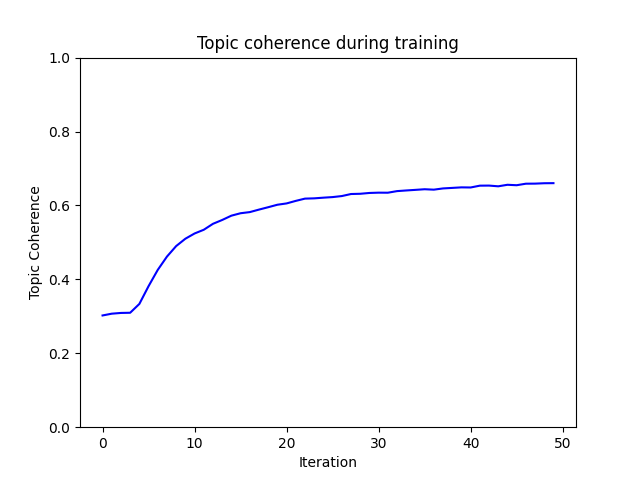
\includegraphics[width= \linewidth]{figures/pachinko_training.PNG}
	\caption{Topic coherence during training of the taxonomy-topic model.}
	\label{fig:pachinko_train}
\end{figure}

\autoref{tab:pachinko_mid_topics} gives an overview of how the taxonomy topics in the third layer of the taxonomy-topic model, are connected to the fourth layer topics that were generated by the model.
Some of these connections make a lot of sense, such as the 'Økonomi' (Economy) topic which has the three filler\vejleder{explain filler} topics: 79, 75, and 42, which consists of words with little semantic value, and two topics which are about money: 74 and 9.
However not all the connections\vejleder{the connections make er understreget} make as much sense as these. 
For example, the 'Kriminalitet' (Crime) topic has two filler topics: 42 and 75, one topic about economy: 60, one topic about politics: 8, and one topic about sports: 86.
See \autoref{tab:pachinko_topics}, for more details on the top words within each of these topics.
\vejleder{uddyb gerne}
Having the layered structure of the \gls{pam} gives many possibilities for recommending new articles to readers.
There is the possibility of exploring the similarity of taxonomies at the same layer and using this to recommend new articles with similar subjects.
For example, if an article is about 'Miljø' (environment) similar taxonomies might be 'Natur' (nature) and possibly 'Etik' (ethics), 'Trafik' (traffic), and 'Energi' (energy).

\begin{table*}[h]
	\centering
	\caption{Top 10 words of selected topics from our taxonomy-topic model. Labels have been manually added to the topics to increase readability.}
	\label{tab:pachinko_selected_topics}
	\begin{tabular}{c | c | c}
		Topic & Label & Top 10 words \\
		\hline
		8 & politics & venstre, valg, valget, partiet, partier, parti, stemmer, mette, politik, regering \\
		9 & money & procent, viser, tal, antallet, milliarder, pct, seneste, penge, millioner, indland \\
		19 & filler & mig, maske, du, folk, synes, ting, faktisk, nogen, altid, tror \\
		21 & university & unge, uddannelse, studerende, gymnasium, elever, uddannelser, universitet, procent, uddannelsen, nordjylland \\
		41 & academic research & universitet, professor, forskere, forskning, forskerne, viser, verden, institut, procent, aarhus \\
		42 & filler & mig, min, mit, ham, aldrig, gik, lille, maske, mine, altid \\
		45 & wildlife & dyr, naturen, natur, ulve, fugle, ulven, arter, dyrene, vilde, ulv \\
		47 & church & kirke, kirken, sognepræst, præst, søndag, koret, gudstjeneste, aften, kor, organist \\
		59 & music concerts & musik, koncert, sange, spiller, koncerter, band, koncerten, festival, musikken, publikum \\
		60 & buisness & virksomheden, millioner, a, direktør, procent, medarbejdere, selskabet, overskud, ansatte, virksomhed \\
		69 & primary school & elever, unge, skole, eleverne, skolen, skoler, klasse, børn, folkeskolen, lærere \\
		74 & elder care & ældre, borgere, kommunen, millioner, penge, nordjylland, plejehjem, borgerne, kommunens, budget \\
		75 & filler & du, din, dig, dit, altsa, dine, maske, nemlig, bruge, hvordan \\
		79 & filler & mig, min, hendes, hende, rigtig, arige, altid, arbejde, mor, mine \\
		86 & sports & handbold, mors, thy, hold, kamp, sæson, kampe, kampen, point, holdet \\
	\end{tabular}
\end{table*}


\begin{table*}[h]
	\centering
	\caption{IDs of the 5 most occurring fourth layer topics for each third layer topic from the pachinko model. See Appendix \autoref{tab:pachinko_topics} for the most occurring words for each ID.}
	\label{tab:pachinko_mid_topics}
	\begin{tabular}{c | c | c | c | c | c}
		Taxonomy Name & Top 5 Topic IDs & Taxonomy Name & Top 5 Topic IDs & Taxonomy Name & Top 5 Topic IDs \\ \hline
		Danmark & 8, 42, 82, 59, 79 & Udland & 42, 79, 59, 8, 32 & Kultur & 9, 42, 79, 19, 8 \\
		Landbrug & 42, 79, 8, 9, 19 & Kriminalitet & 42, 75, 60, 8, 86 & Socialstof & 42, 9, 79, 86, 8 \\
		Arbejdsmarked & 42, 79, 59, 8, 9 & Økonomi & 79, 75, 74, 42, 9 & Sundhed & 8, 32, 42, 9, 19 \\
		Politik & 42, 75, 9, 19, 74 & Musik & 75, 42, 59, 11, 79 & Sport & 42, 75, 8, 59, 52 \\
		Bolig & 75, 42, 86, 79, 8 & Videnskab & 42, 8, 52, 79, 19 & Trafik & 42, 74, 8, 52, 32 \\
		Erhverv & 42, 8, 59, 32, 79 & Uddannelse & 42, 9, 75, 32, 74 & Energi & 42, 8, 79, 19, 86 \\
		Ulykker & 42, 75, 9, 79, 32 & Fritid & 42, 8, 75, 82, 79 & Socialt & 42, 75, 79, 59, 9 \\
		Dyr & 86, 42, 79, 52, 9 & Natur & 42, 52, 9, 32, 79 & Miljø & 8, 42, 75, 52, 59 \\
		Familie & 79, 8, 42, 59, 32 & Politi & 42, 75, 79, 8, 59 & Byggeri & 75, 42, 79, 77, 59 \\
		Etik & 79, 42, 8, 86, 74 & Religion & 42, 79, 8, 59, 32 & Kommunalvalg & 42, 8, 75, 79, 32 \\
		Nordjyske Plus & 42, 86, 9, 79, 74 & DF & 42, 8, 59, 52, 19 & & \\
	\end{tabular}
\end{table*}

